% CVPR 2023 Paper Template
% based on the CVPR template provided by Ming-Ming Cheng (https://github.com/MCG-NKU/CVPR_Template)
% modified and extended by Stefan Roth (stefan.roth@NOSPAMtu-darmstadt.de)

\documentclass[10pt,twocolumn,letterpaper]{article}

%%%%%%%%% PAPER TYPE  - PLEASE UPDATE FOR FINAL VERSION
% \usepackage[review]{cvpr}      % To produce the REVIEW version
\usepackage{cvpr}              % To produce the CAMERA-READY version
% \usepackage[pagenumbers]{cvpr} % To force page numbers, e.g. for an arXiv version

% Include other packages here, before hyperref.
\usepackage{graphicx}
\usepackage{amsmath}
\usepackage{amssymb}
\usepackage{booktabs}
\usepackage[none]{hyphenat}
\usepackage{array}


% It is strongly recommended to use hyperref, especially for the review version.
% hyperref with option pagebackref eases the reviewers' job.
% Please disable hyperref *only* if you encounter grave issues, e.g. with the
% file validation for the camera-ready version.
%
% If you comment hyperref and then uncomment it, you should delete
% ReviewTempalte.aux before re-running LaTeX.
% (Or just hit 'q' on the first LaTeX run, let it finish, and you
%  should be clear).
\usepackage[pagebackref,breaklinks,colorlinks]{hyperref}


% Support for easy cross-referencing
\usepackage[capitalize]{cleveref}
\crefname{section}{Sec.}{Secs.}
\Crefname{section}{Section}{Sections}
\Crefname{table}{Table}{Tables}
\crefname{table}{Tab.}{Tabs.}


%%%%%%%%% PAPER ID  - PLEASE UPDATE
\def\cvprPaperID{*****} % *** Enter the CVPR Paper ID here
\def\confName{CVPR}
\def\confYear{2023}


\begin{document}

% <><><><><><><><><><><><><><><><><><><><><><><><><><><><><><><><><><><><><><><><>
%                             TITLE AND AUTHORS
% <><><><><><><><><><><><><><><><><><><><><><><><><><><><><><><><><><><><><><><><>
\title{Motion Diffusion Model to Denoising Diffusion GAN: Efficient Motion Sampling}

\author{
    Ronald Campos\\
    University of Central Florida\\
    4000 Central Florida Blvd, Orlando, FL 32816\\
    {\tt\small roncamposj@knights.ucf.edu}
    \and
    Muhammad Asad Haider\\
    University of Central Florida\\
    4000 Central Florida Blvd, Orlando, FL 32816\\
    {\tt\small haider24@knights.ucf.edu}
    \and
    Suneet Tipirneni\\
    University of Central Florida\\
    4000 Central Florida Blvd, Orlando, FL 32816\\
    {\tt\small suneet.tipirneni@knights.ucf.edu}
    \and
    Stefan Werleman\\
    University of Central Florida\\
    4000 Central Florida Blvd, Orlando, FL 32816\\
    {\tt\small stefanwerleman@knights.ucf.edu}
}


\maketitle

% <><><><><><><><><><><><><><><><><><><><><><><><><><><><><><><><><><><><><><><><>
%                                  ABSTRACT
% <><><><><><><><><><><><><><><><><><><><><><><><><><><><><><><><><><><><><><><><>
\begin{abstract}
    All existing human motion diffusion models use the standard diffusion process which yields high 
    quality samples. However, the standard process for these models can be inefficient. These are one of
    the challenges with the learning trilemma and this works concerns embedding an existing motion diffusion 
    model into denoising diffusion GANs to create a hybrid architecture of the motion diffusion model. This 
    new hybrid model will satisfy the learning trilemma, thus improving the sampling speed when training and generating a motion sample.
    \url{https://github.com/CAP6412-Group-4/denoising-diffusion-gan}
\end{abstract}


% <><><><><><><><><><><><><><><><><><><><><><><><><><><><><><><><><><><><><><><><>
%                                  INTRODUCTION
% <><><><><><><><><><><><><><><><><><><><><><><><><><><><><><><><><><><><><><><><>
\section{Introduction}
\label{sec:intro}

Deep generative models had many breakthroughs in past years. Many applications have been built such as: 
image synthesis, inpainting, image classification, segmentation, point clouds, and audio. One of the latest developments with 
these models is the ability to generate human motions based on text inputs. However, there are three key requirements 
that generative models cannot satisfy: high-quality sampling, mode coverage and diversity, and fast sampling. 

\subsection{Human Motion Diffusion Model}

The human motion diffusion model (MDM) is a generative model that generates human motions. Given a text prompt 
that describes the motion the applicatin would output a video that shows a skeleton figure perfoming the 
action that was described in the text prompt. 

The MDM can generate high quality motion samples and achieve good mode coverage. 
However, the generative model for MDM requires a great amount of timesteps in the reverse process which means 
that the current MDM does not satisfy the fast sampling in the learning trilemma (Figure \ref{fig:intro-0}). 

\subsection{Improving Sampling}

Proposed by Xiao et al. (2022), the Denoising Diffusion GAN (DDGAN) is a novel generative model that utilizes 
GANs to satisfy all three requirements of the generative learning trilemma. Specifically, the usage of 
conditional GANs is what decreases the timesteps during sampling (Figure \ref{fig:intro-1}). As a result, training is a lot faster 
compared to traditional diffusion models. Furthermore, this enhancement prevents issues such as collapse and 
overfitting \cite{Xiao22}.

\begin{figure*}[h!]    
    \centering
    \fbox{
    \begin{tabular}{cc}
        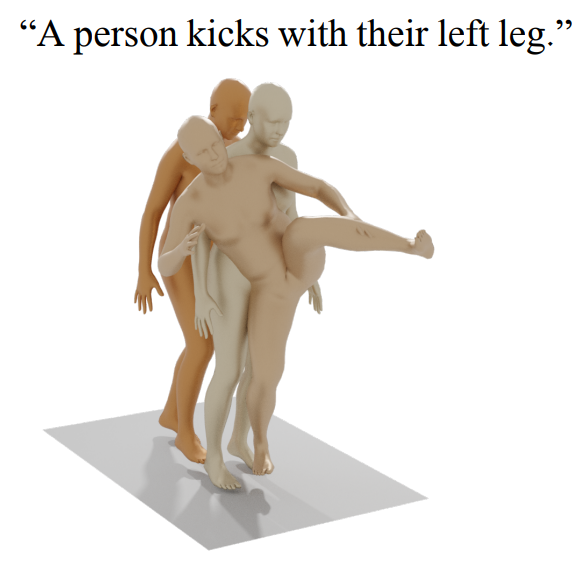
\includegraphics[width=0.3\textwidth]{imgs/introduction/mdm.png}
        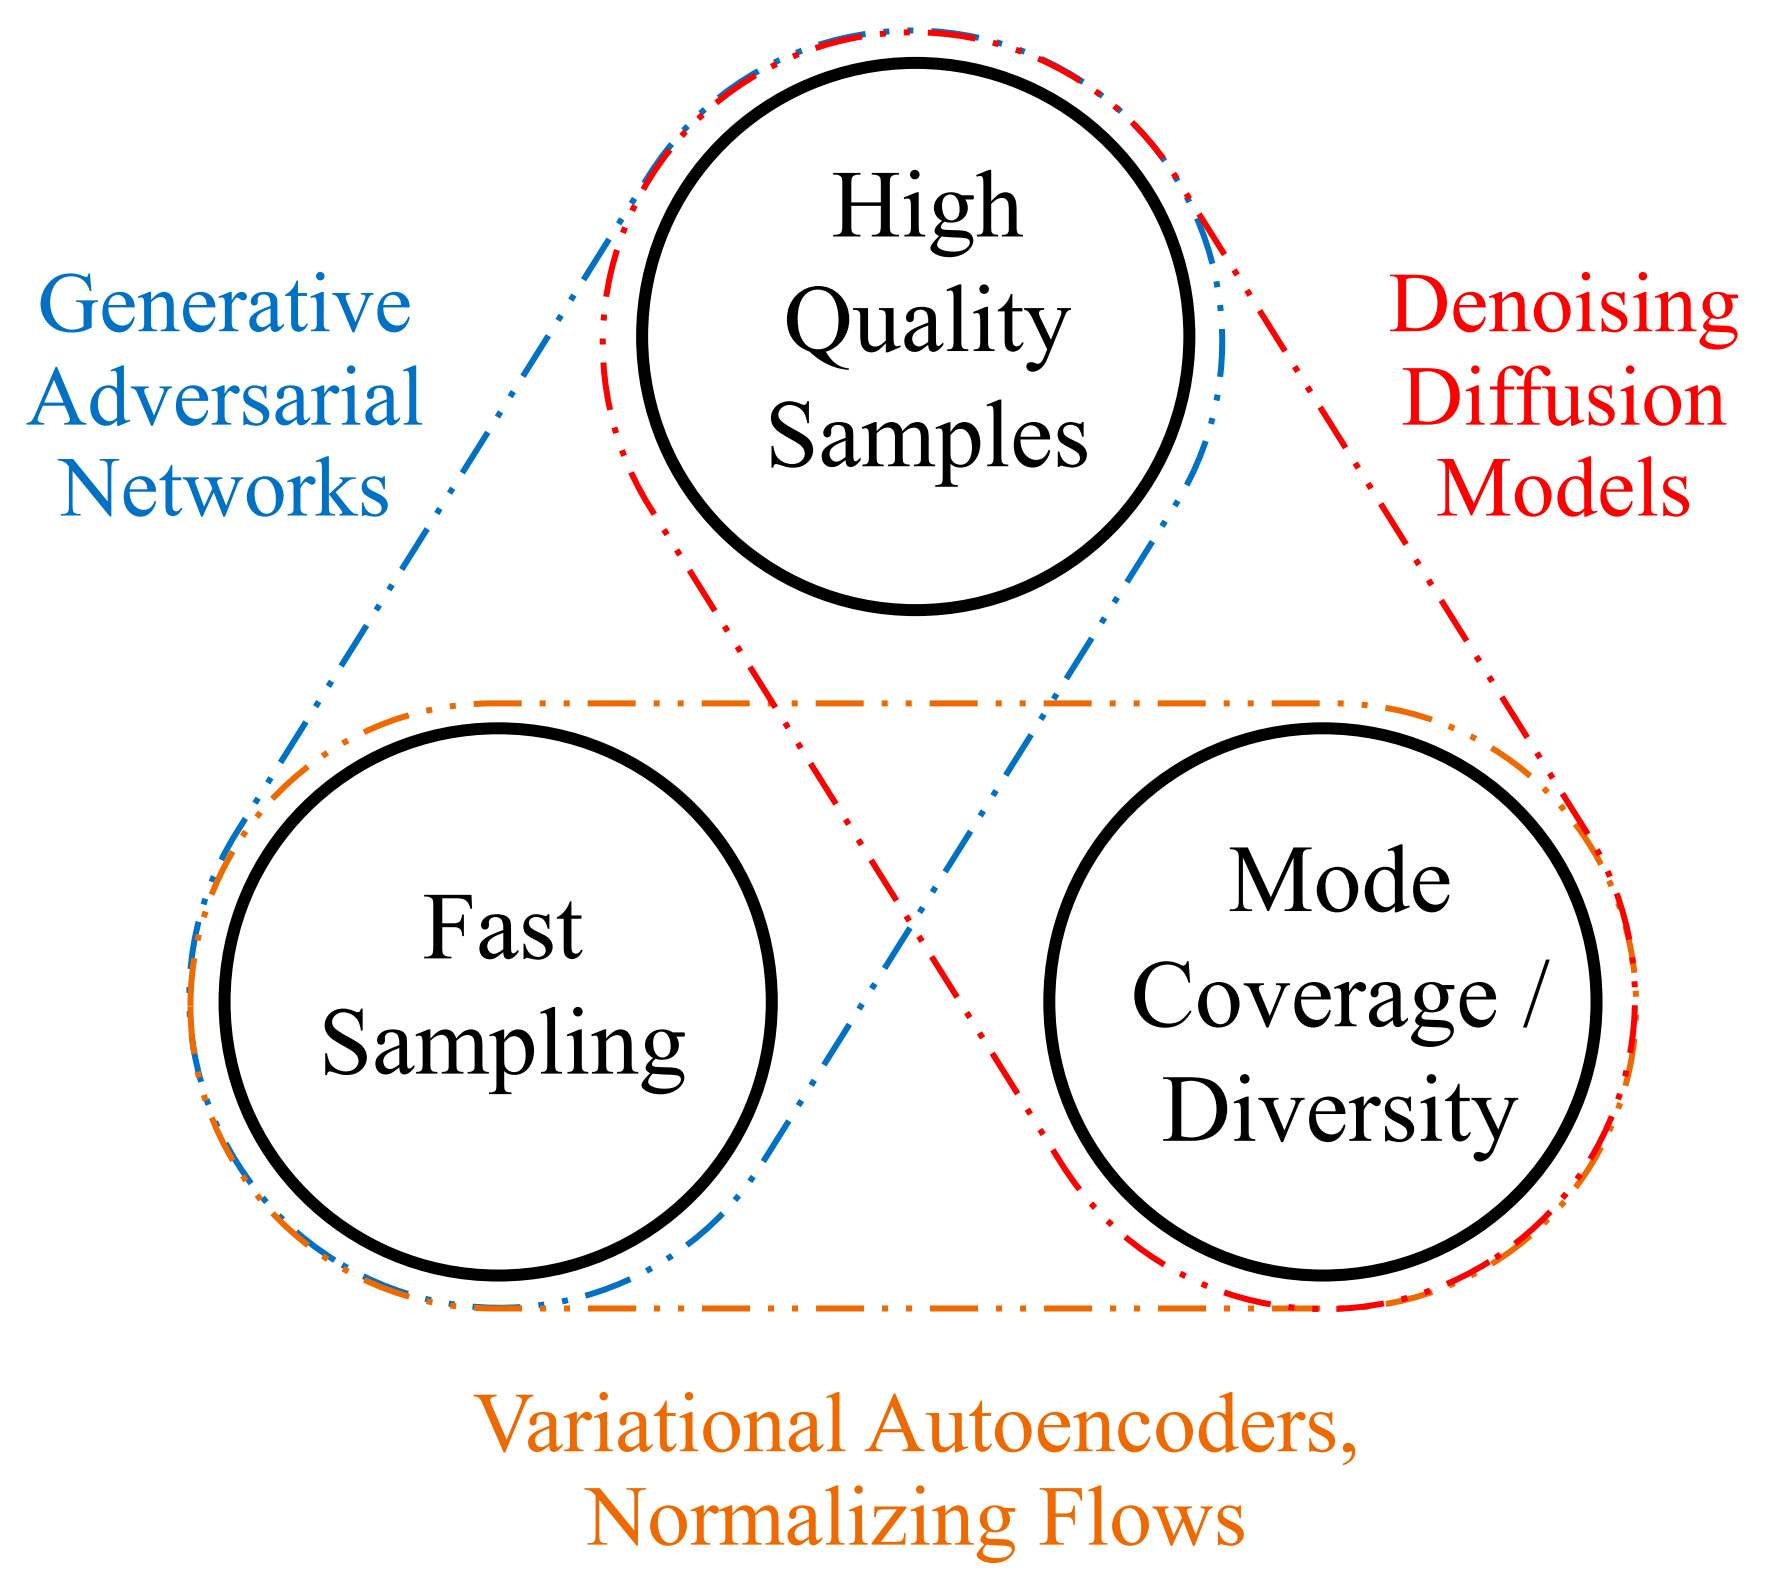
\includegraphics[width=0.3\textwidth]{imgs/introduction/learning_trilemma.png}
    \end{tabular}
    }
    \caption{Motion synthesise and the Generative learning trilemma \cite{Tevet23} \cite{Xiao22}}    
    \label{fig:intro-0}
\end{figure*}

\subsection{Integrating Motion Diffusion Model Into DDGAN}

Initially, DDGAN was not designed for human motion data, but can be modified to do so. Specifically, DDGAN 
is built to handle image loss not motion or geometric loss which are complete different from each other. 
Therefore, we had to modify the DDGAN so that it can handle motion loss before integrating MDM to it. As for MDM, we needed to 
remove some existing logic in the current worklflow to make the final addition of the DDGAN (Section \ref{sec:method}). 

% <><><><><><><><><><><><><><><><><><><><><><><><><><><><><><><><><><><><><><><><>
%                                  RELATED WORK
% <><><><><><><><><><><><><><><><><><><><><><><><><><><><><><><><><><><><><><><><>
\section{Related Work}
\label{sec:related-work}

\subsection{Human Motion Diffusion Model}

\subsection{Denoising Diffusion GANs}


% <><><><><><><><><><><><><><><><><><><><><><><><><><><><><><><><><><><><><><><><>
%                                  METHOD
% <><><><><><><><><><><><><><><><><><><><><><><><><><><><><><><><><><><><><><><><>
\section{Method}
\label{sec:method}

\subsection{Motion Diffusion Model Integration}
As implied by the title and previous text, our model aims to apply the sampling gains provided by \cite{Xiao22}. However in doing this we needed to make fundamental changes to how the MDM is constructed. More specifically, The model needs to ingest the latent $z$ variable as decribed in \cite{Xiao22}. Secondly, the DDGAN model needs to adjust it's dimensionality to take in frames of joint positions rather than taking a single image frame dimensions as input.

\subsubsection{MDM Modifications}

The MDM model as-provided already provides a fantastic framework for a generator model. Most of the model can remain intact however additions were made to make the model more versatile. The primary change occurs with the introduction of the latent $z$ variable. This variable is the mapping variable used for conditional score networks and allows the MDM model to sample from a non-normal distribution \cite{xiao2022tackling}. The latent $z$ variable is added to the other inputs described in \cite{Tevet23}. For our our purposes we use different $z$ mapping layers that discard image-specific normalization and change output channels to match the desired dimenions of the humanml dataset.  Our resulting MDM architecture is shown if figure \ref{fig:modified-mdm]}. \par

\subsubsection{DDGAN Modifications}\label{sec:ddgan-mod}

As for the denoising-diffusion-GAN (ddgan). We fixed the image dimension of the model to $120$. This is done to align with the dimensionality used in \cite{Guo_2022_CVPR}. Instead of using the generator provided by \cite{Xiao22} we replace the generator with our modified MDM architecture. As a result we are effectively using the discrminator to discriminate against samples our MDM model generates. \par 

\begin{figure*}[h!t]
	\centering
	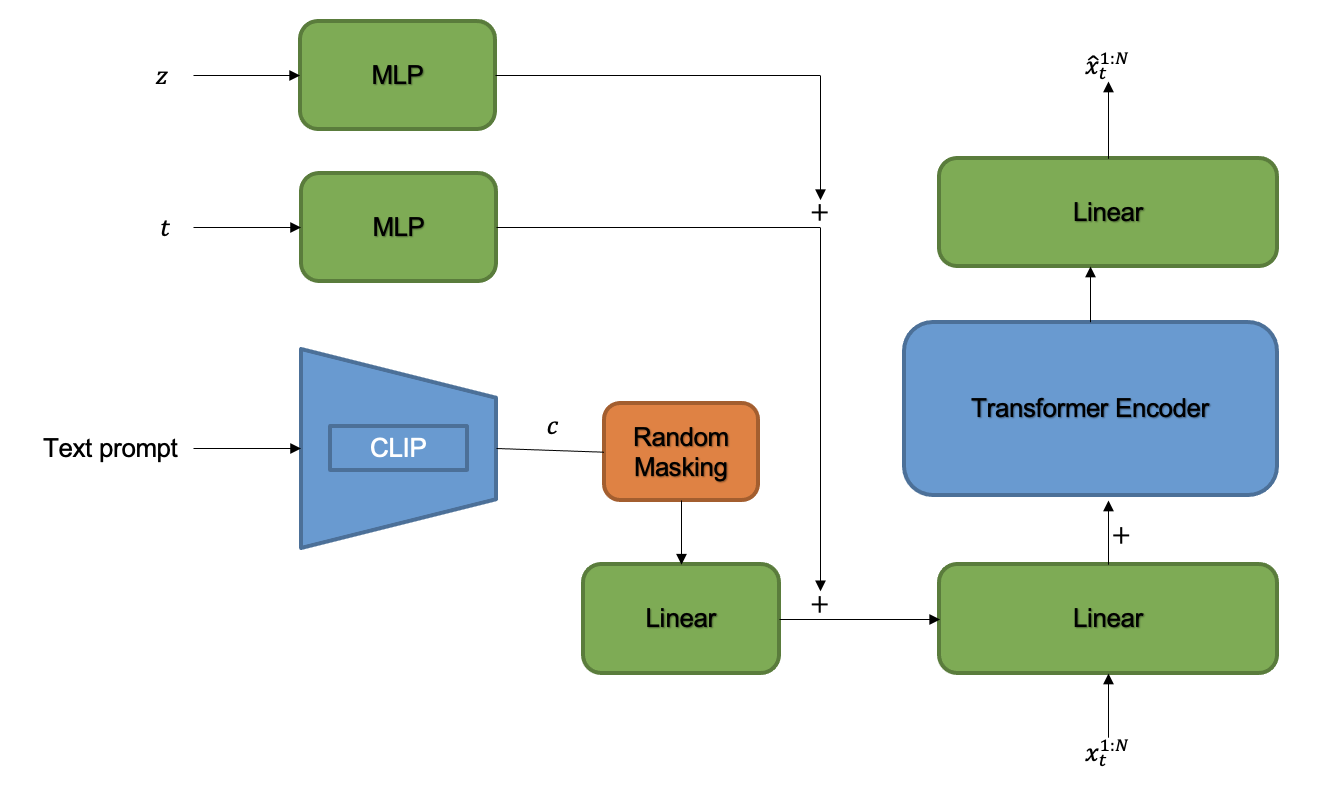
\includegraphics[width=0.8\textwidth]{imgs/modified-MDM.png}
	\caption{Our modified MDM architecture based on \cite{Tevet23}, we introduce the latent $z$ variable by adding it with the timestep condition and the text prompt condition $c$}
	\label{fig:modified-mdm]}
\end{figure*}

\subsection{Adapting The Loss}

As described in \ref{sec:ddgan-mod} we are using the discriminator to validate the values given from our generator. The discrinator offers us adversarial loss, however, this loss along is not sufficient for our generator. Our generate being an MDM requires additional losses to produce high-quaility outputs. For this we borrow the geometric losses described in \cite{Tevet23}. Even though adversarial loss is not sufficient to properly to the model alone, it is still needed as a loss to propogate. As a result, we simply add adversarial loss to the geometric losses which results in equation \ref{eq:losses}.

\begin{equation}\label{eq:losses}
	\mathcal{L}_{all} = \lambda_{adv}\mathcal{L}_{adv} + \lambda_{pos}\mathcal{L}_{pos} + \lambda_{vel}\mathcal{L}_{vel} + \lambda_{foot}\mathcal{L}_{foot} 
\end{equation}

% <><><><><><><><><><><><><><><><><><><><><><><><><><><><><><><><><><><><><><><><>
%                                  EXPERIMENTS
% <><><><><><><><><><><><><><><><><><><><><><><><><><><><><><><><><><><><><><><><>
\section{Experiments}
\label{sec:experiments}
Our implementation of MDM-2-Diffgan (M2D) is applied for the task of text-to-motion generation. We trained our models with T = 4 noising steps, 
using a cosine noise schedule. Experiments were conducted using the Newton cluster which employs two NVIDIA V100 GPUs per node. During the 
training process of our models, we conducted experiments with varying numbers of epochs, ranging from 200 to 1200, and determined that the 
most optimal results were achieved with fewer epochs, specifically at the lower end of the range. Training on this lower range took approximately
about a day.
\\

The HumanML3D dataset, which was also used by \cite{Tevet23}, was employed in our text-to-motion generation task. HumanML3D \cite{Guo_2022_CVPR}
is a combination the HumanAct12 \cite{guo2020action2motion} and Amass \cite{Amass} datasets, which covers a broad range of activities, such as 'jumping', 
dancing', and certain other acrobatics. The dataset contains 14,616 motion clips and 44,970 text descriptions.
\\

Our models were trained with a batch size of 128. Our generator used a learning rate of 0.0015, while the learning rate of the discriminator was slightly 
larger at 0.0001. We employed the same parameters as \cite{Tevet23} did with the transformer encoder and used that as our generator: 8 layers, an embedding 
dimension of 512, a GELU activation function, and dropout with a rate of 0.1. The discriminator uses an embedding dimension of 128, to go along with its 6 
downsampling blocks. Its final output is 256 channels. Both the generator and discriminator use a softplus loss function, which is a smooth aproximation 
of the ReLU. We conducted experiments with varying weights $\lambda$ for the geometric losses, but observed that our results were unsatisfactory when 
$\lambda > 0$, which aligns with the findings reported in \cite{Tevet23}. Geometric losses are already represented in the HumanML3D ensemble, thus it is
justifiable to omit them during training.
% <><><><><><><><><><><><><><><><><><><><><><><><><><><><><><><><><><><><><><><><>
%                                  RESULTS
% <><><><><><><><><><><><><><><><><><><><><><><><><><><><><><><><><><><><><><><><>
\section{Results}
\label{sec:results}
\subsection{Qualitative Results}

Our qualitative findings illustrate that our model is capable of most generations that MDM can perform, but with a few discrepancies we should note. In the 
final seconds of our generations, our results will generally exhibit a floor sliding effect, where after following the text prompt, the plane beneath the
figure will shift. This is not the same as the foot contact sliding effect, since by this point the prompt has been completed and the generation is just 
standing still. This effect is not present in the MDM generations, and we believe that this is due to the fact that the MDM model is trained on a dataset
that does not contain this effect. We believe this is a result of some model instability, but at this time are unable to pinpoint the exact cause.
\\

Taking this into consideration, we maintain our conviction that the generations excel in capturing what the text-prompts indicate. We believe that the 
distribution of HumanML3D is effectively captured by MDM-2-Diffgan, where we observed a favorable range of variability in generations. In the future, 
we would like to perform a user study in order to obtain less biased interpretaions of our results. 

\begin{figure}[h!]    
    \centering
    \fbox{
    \begin{tabular}{cc}
        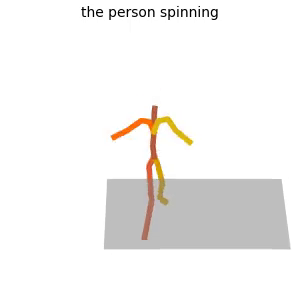
\includegraphics[width=.2\textwidth]{imgs/spinning/frame_30.png}&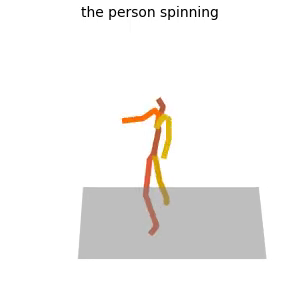
\includegraphics[width=.2\textwidth]{imgs/spinning/frame_50.png}\\
        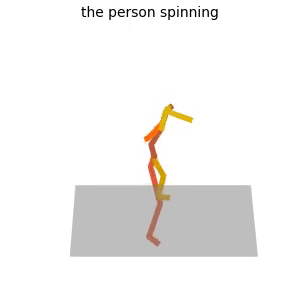
\includegraphics[width=.2\textwidth]{imgs/spinning/frame_60.png}&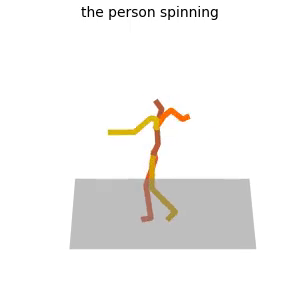
\includegraphics[width=.2\textwidth]{imgs/spinning/frame_80.png}\\
        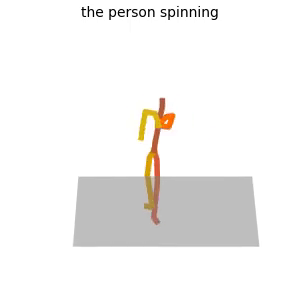
\includegraphics[width=.2\textwidth]{imgs/spinning/frame_100.png}&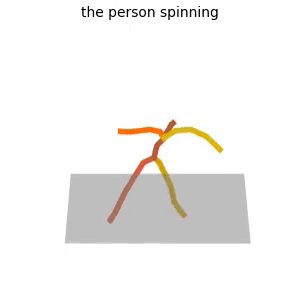
\includegraphics[width=.2\textwidth]{imgs/spinning/frame_110.png}\\
    \end{tabular}
    }
    \caption{The shows a person in the act of spinning. (Subject to change)}    
    \label{fig:quant}
\end{figure}
% temporarily adding newpage until I find a better solution
\newpage
\subsection{Quantitative Results}

As a quick reminder, let's recall the metrics we use to evaluate our model. We use the R-Precision score, which measures the similarity between the generated
motion and the text prompt. FID and Multimodal Distance scores measures the similarity between the generated motion and the real motion. Lastly, Diversity 
measures the variability between the generated motions.
\\

We compare our results with the results of \cite{Tevet23} and other motion generation models, which are shown in Table \ref{tab:metrics} 
and \ref{tab:metrics2}. We can observe that MDM-2-Diffgan performs fairly well when compared to MDM. While we don't set the state-of-the-art
the state of the art in any of the metrics, we are able to achieve a higher R-Precision score than MDM. Also we have a comparable diversity and Multimodality
scores, which is a good sign that our model is able to capture the distribution of the HumanML3D dataset. We observe a poor FID score when
compared to MDM. 

\begin{table}[h]
    \centering
    \begin{tabular}{|p{1.4cm}|p{1.8cm}|p{1.5cm}|c|c|c|c|c|c|}
    \hline Method & $\begin{array}{l}\text { R Precision } \\
    \text { (top } 3 \text { )↑ }\end{array}$ & FID $\downarrow$ & $\begin{array}{c}\text { Multimodal } \\
    \text { Dist } \downarrow\end{array}$ \\
    \hline Real & $0.797_{ \pm .002}$ & $0.002_{ \pm .000}$ & $2.974_{ \pm .008}$ \\
    \hline JL2P & $0.486_{ \pm .002}$ & $11.02_{ \pm .046}$ & $5.296_{ \pm .008}$ \\
    \hline $\mathrm{T} 2 \mathrm{M}$ & $0.740_{ \pm .003}$ & $1.067_{ \pm .002}$ & $3.340_{ \pm .008}$ \\
    \hline MDM & $0.611_{ \pm .007}$ & $0.544_{ \pm .044}$ & $5.566_{ \pm .027}$ \\
    \hline M2D & $0.698_{ \pm .007}$ & $2.44_{ \pm .429}$ & $6.353_{ \pm .076}$ \\
    \hline
    \end{tabular}
    \caption{MDM-2-Diffgan accomplishes a higher R-Precision score than MDM, but a substantially lower FID score.}
    \label{tab:metrics}
\end{table}
\begin{table}[h]
    \begin{tabular}{|p{2cm}|p{2cm}|p{2cm}|c|c|c|c|c|c|}
        \hline Method & Diversity $\rightarrow$ & Multimodality $\uparrow$ \\
        \hline Real & $9.503_{ \pm .065}$ & - \\
        \hline JL2P & $7.676_{ \pm .058}$ & - \\
        \hline $\mathrm{T} 2 \mathrm{M}$ & $9.188_{ \pm .002}$ & $2.090_{ \pm .083}$ \\
        \hline MDM & $9.559_{ \pm .086}$ & $2.799_{ \pm .072}$ \\
        \hline M2D & $9.416_{ \pm .057}$ & $2.671_{ \pm .025}$ \\
        \hline
        \end{tabular}
    \caption{We observe a similarity of around 0.1 for both metrics between MDM and MDM-2-Diffgan.}
    \label{tab:metrics2}
\end{table}

\newpage

We also perform a speed test, where we measure the time it takes MDM-2-Diffgan to generate motions. We perform 
three experiments where we generate motions with: 1 sample $s$ and 1 repetition $r$, 3 samples $s$ and 1 repetition $r$, and 10 samples 
$s$ and 3 $r$. From the results in Table \ref{tab:time}, we can observe that it takes MDM considerably longer to generate motions 
than Motion-2-Diffgan. We can see that MDM takes 16.58 seconds to generate 1 sample and 1 repetition, while M2D takes 0.22 seconds. 
What is noteworthy though, is how both models scale in as we increase the number of samples and repetitions. MDM takes 105.14 seconds 
to generate 10 samples and 3 repetitions, whereas M2D only takes 0.64 seconds. This is a significant improvement in time, and shows that 
MDM-2-Diffgan is able to scale much more effectively than MDM. 

\begin{table}[]
    \centering
    \begin{tabular}{|c|ccc|}
    \hline
    Method & \multicolumn{1}{c|}{1s \& 1r} & \multicolumn{1}{c|}{3s \& 1r} & 10s \& 3r \\ \hline
           & \multicolumn{3}{c|}{Seconds}                                              \\ \hline
    MDM    & \multicolumn{1}{c|}{16.58}    & \multicolumn{1}{c|}{18.28}    & 105.14    \\ \hline
    M2D    & \multicolumn{1}{c|}{0.22}     & \multicolumn{1}{c|}{0.31}     & 0.64      \\ \hline
    \end{tabular}
    \caption{Our samples generated around 100x faster than those from MDM.}
    \label{tab:time}
\end{table}

% temporarily adding newpage until I find a better solution
\newpage

% <><><><><><><><><><><><><><><><><><><><><><><><><><><><><><><><><><><><><><><><>
%                           ADDITIONAL APPLICATIONS
% <><><><><><><><><><><><><><><><><><><><><><><><><><><><><><><><><><><><><><><><>
\section{Additional Applications}
\label{sec:additional-applications}

Once our hybrid motion diffusion model was complete and generating results, we want to see how we can
leverage the motion samples for other applications. 

\subsection{Using Motion Samples for Person Image Synthesis (PIDM)}

\begin{figure}[h]
    \centering
    \fbox{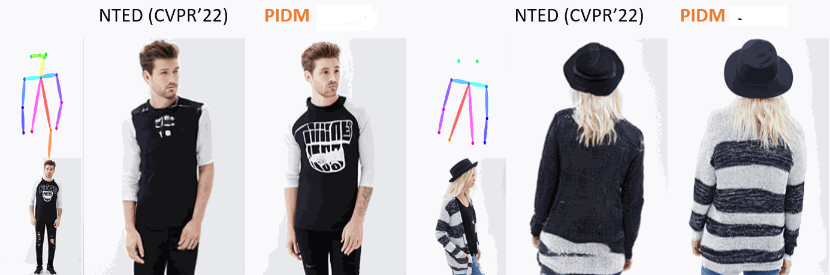
\includegraphics[width=0.47\textwidth]{imgs/pidm/pidm_0.png}}

    \caption{Image sample of the pose-guided image synthesis.}
    \label{fig:pidm-0}
\end{figure}

We wanted to use the produced motion samples from our hybrid as target poses or position to generate 
photorealistic images of humans \cite{Bhunia23}. There are several pose-guided person image generation
models but this model proposed by Ankan Bhunia et al. (2023) utilizes a denoising diffusion model to
generate the image samples (Figure \ref{fig:pidm-0}).

The process goes as follows: given a target pose in the form of a skeleton and a reference image 
of a person, in each diffusion step the model generates a sharper version of the final image until it
reaches \emph{T} total diffusion steps (Figure \ref{fig:pidm-1}). The target pose is a color-coded where
each color represents a joint or body of the person in the final sampled image. For instance, the green 
joints in the skeleton represents the position of the head, the yellow shoulder represents the left shoulder 
position, and so on.

\begin{figure}[h]
    \centering
    \fbox{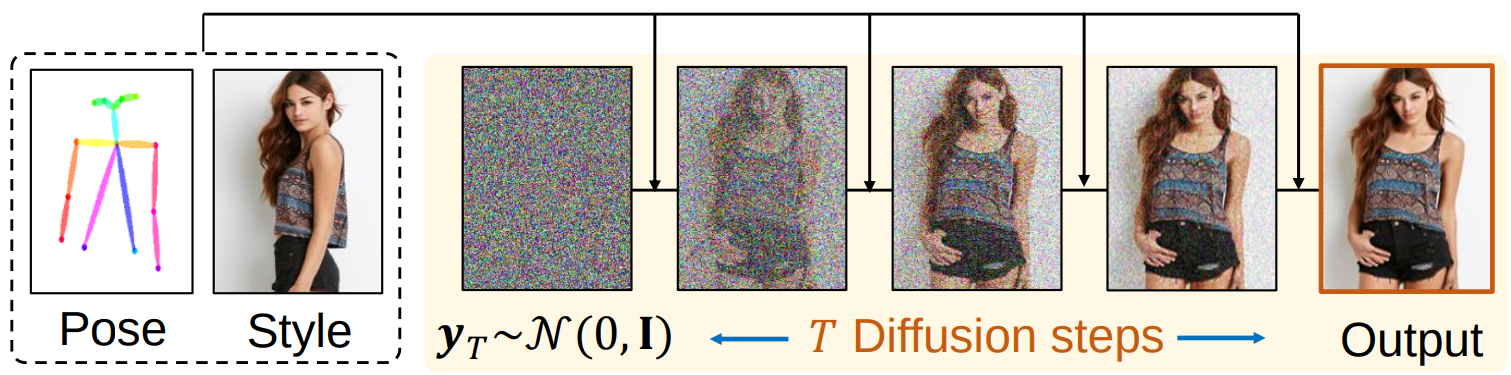
\includegraphics[width=0.47\textwidth]{imgs/pidm/pidm_1.png}}

    \caption{General workflow for the Person Image Synthesis Denoising Diffusion Model.}
    \label{fig:pidm-1}
\end{figure}

In Figure \ref{fig:quant}, our motion diffusion model produces skeletons that perform certain actions. 
However, our skeleton images are color-coded differently and are missing the head position of the person 
generated. First step was to determine a mapping from the motion diffusion skeleton to the correct color-codes 
for PIDM. Next, is to take the target pose image sample and create a numpy array representation of it. The PIDM 
diffusion model expected an input shape of 256x256x20 where the first 3 channels represent the pose skeleton 
while the remaining 17 skeletons are gaussian keypoint maps. We were only able to reproduce the first 3 channels 
from our MDM skeleton pose and created the remaining 17 channels with values of zeros.

\begin{figure}[h]
    \centering
    \fbox{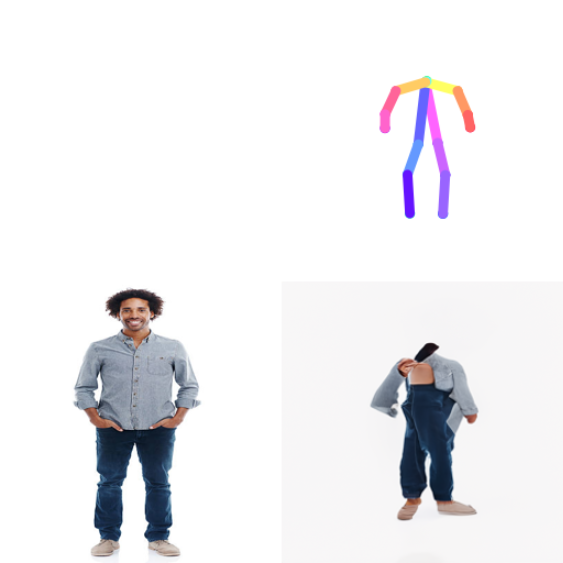
\includegraphics[width=0.45\textwidth]{imgs/pidm/pidm_2.png}}

    \caption{The target pose generated by our motion diffusion model was suppose to represent a 
    person who is facing their back towards us.}
    \label{fig:pidm-2}
\end{figure}


After, getting our custom pose image to the appropraite array representation for the diffusion model in PIDM, 
we were able to finally test it and generate a sample pose-guided image. Unfortunately, the sampled image 
did not produce the results we expected as the final person image appeared to be disfigured (Figure \ref{fig:pidm-2}). 
This is probably due to the absence of the 17 guassian keypoint channels in our target pose skeleton and 
is also due to the missing head position in the target pose.

% TODO: Ron and Asad mentioned how long PIDM took to generate this sample image.

% <><><><><><><><><><><><><><><><><><><><><><><><><><><><><><><><><><><><><><><><>
%                         CONCLUSION AND FUTURE WORKS
% <><><><><><><><><><><><><><><><><><><><><><><><><><><><><><><><><><><><><><><><>
\section{Conclusion and Future Works}
\label{sec:conlusion}

% <><><><><><><><><><><><><><><><><><><><><><><><><><><><><><><><><><><><><><><><>
%                               REFERENCES
% <><><><><><><><><><><><><><><><><><><><><><><><><><><><><><><><><><><><><><><><>
\newpage
{\small
\bibliographystyle{ieee_fullname}
\bibliography{egbib}
}

% TODO: Thought it would better to include the DDGAN in the appendix. Let me know if we need this.

\appendix
\section{Appendix}

\begin{figure}[h]
    \centering
    \fbox{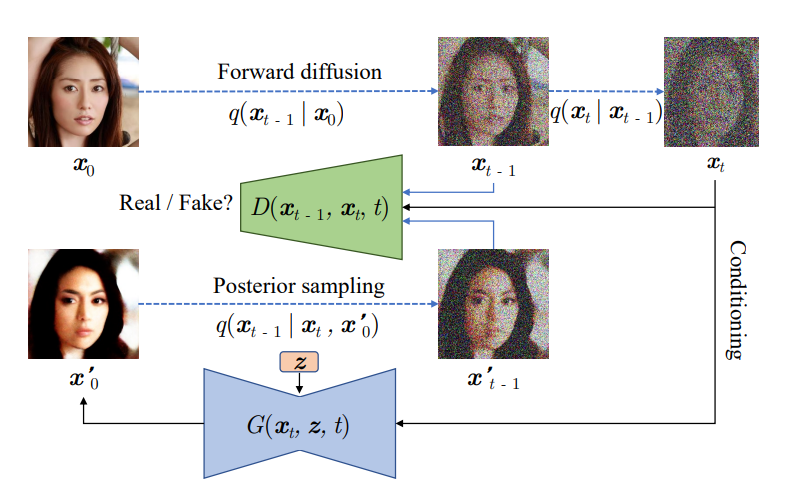
\includegraphics[width=0.47\textwidth]{imgs/introduction/ddgan.png}}

    \caption{Denoising Diffusion GANs Architecture \cite{Xiao22}.}
    \label{fig:intro-1}
\end{figure}


\end{document}
